\chapter{Gravitational waves associated with gamma-ray bursts}\label{ch:grb}

\section{Gamma-ray bursts}\label{sec:grb-astro}

\Acp{GRB} are short, energetic bursts of gamma rays in the MeV range, first discovered in 1967~\citep{Klebesadel_1973}.
Observations throughout the following decades revealed that \acp{GRB} could be classified based on duration and spectral hardness~\citep{Kouveliotou_1993}.
This classification has become the most used to describe \acp{GRB}: long-soft bursts last $\gtrsim2$ s and have soft emission spectra, i.e. lacking in higher energy photons, while short-hard bursts last $\lesssim2$ s and had harder emission spectra.
It is believed that the ultra-relativistic jets required to produce \acp{GRB} come from either black holes~\citep{Woosley_1993} or magnetars~\citep{Dai_1998}.

A multitude of models have been proposed throughout the decades to explain the origins of \acp{GRB}.

Photometry and spectroscopy data provide evidence that long \acp{GRB} originate from \acp{CCSN}, whereas short \acp{GRB} are believed to be associated with compact binary mergers, such as the \ac{BNS} merger GW170817~\citep{gw170817_grb}.

In the case of long \acp{GRB}, some models predict the emission of \acp{GW} as a result of asymmetries in the core-collapse phase.
Such \acp{GW} would be short, lasting less than a second.
Extreme emission models predict a wide variety of signals, often longer in duration.
Matter surrounding the remnant of a \ac{CCSN} forms an accretion disk, in which turbulent behavior can arise.
For instance, instabilities in the accretion disk can lead to the formation of a clump of matter which can then migrate inwards, shedding angular momentum in the form of gravitational waves.

\section{GW searches}\label{sec:grb-searches}

In 2017, the first binary neutron star merger GW170817 was detected by advanced LIGO and Virgo, immediately accompanied by the detection of a relatively low-luminosity gamma-ray burst GRB170817A by Fermi \ac{GBM} two seconds later~\citep{gw170817}.
This prompted a global effort to find an optical, UV, and infrared counterpart that would make up the signature of a kilonova.
The localization provided by the joint detection was sufficient to locate a counterpart near NGC 4993.

\ac{GW} parameter estimation suffers from a degeneracy between distance and orbital plane inclination; increasing the distance of the merger and orienting its orbital plane would both result in a lower \ac{GW} amplitude.
This degeneracy can be broken if either one could be measured externally.
If the joint detection localization were good enough to determine a host galaxy, this would greatly help resolve the distance, however this will more likely require observation of an optical or UV counterpart due to the poor localization provided by current \ac{GRB} and \ac{GW} detectors.
In the case of GW170817, the host galaxy whose redshift was known was used to determine the distance, which then allowed for a more precise measurement of the inclination angle.
A separate analysis using the distance measured from the \ac{GW} detection combined with the known redshift made the first joint \ac{GW}-EM measurement of the Hubble constant, albeit with very large uncertainty due to the small sample size~\citep{gw170817_hubble}.

One of the many unanswered questions surrounding \acp{GRB} pertains to their jet profile, the luminosity as a function of viewing angle (the angle between the observer and the symmetric axis of the jet; the profile is assumed to be axially symmetric and independent of distance).
When information about the jet profile is required, e.g. for making rate estimates for \ac{GRB} detections, the profile is typically modeled as a top-hat (uniform within some opening angle and dropping sharply beyond it) for simplicity, but the true profile may be different.

Determining the viewing angle $\theta_{\mathrm{obs}}$ of a \ac{GRB} is essential for distinguishing between different jet profile models, but it relies on the ability to observe an afterglow emission.
These emissions, ranging from radio to X-rays, follow the prompt emission of $\gamma$-rays and are generated by the interaction between the relativistic outflow and the surrounding medium.
The observation of these afterglows was crucial in improving localization of the \ac{GRB} sources and provided valuable information about the energy scale of the jet, as well as measurements of $\theta_{\mathrm{obs}}$.
The latter came from observing the signature jet break in the afterglow light curve, resulting from the lateral spreading of jet material as it expands; the opening angle can be determined from the timing of the jet break.
However, few jet breaks have been observed for short \acp{GRB}, so existing observations do not place tight constraints on opening angle~\citep{Biscoveanu_2020}.

Joint GW-GRB observations can provide much more information on jet properties~\citep{Mogushi_2019, Farah_2020}.
GRB170817 was orders of magnitude less energetic than most short \acp{GRB}, so it likely would have been ignored in the absence of a \ac{GW} coincidence.
Its low luminosity immediately ruled out an on-axis top-hat jet.
An off-axis top-hat jet was considered unlikely as well because the narrow opening angle predicted for top-hat jets based on theory and past \ac{GRB} measurements only allowed for $\theta_{\mathrm{obs}} \lesssim 10\deg$.
More evidence against an off-axis top-hat model arose when the bright afterglow expected to emerge after $\sim$1 day was not observed.
These observations instead favored a wide-angled, structured jet model for GRB170817.
A structured jet model may refer to any luminosity function that decreases gradually with $\theta_{\mathrm{obs}}$ rather than abruptly, e.g. a Gaussian or power-law with uniform center.
One mechanism that would explain such a model is a cocoon emission, in which the relativistic jet interacts dissipatively with the surrounding merger ejecta, depositing its energy into a cocoon fireball that results in a structured jet~\citep{gw170817_grb}.

The \ac{LIGO}-Virgo collaboration searches for gravitational waves associated with \acp{GRB} detected by Fermi \ac{GBM} and Swift \ac{BAT} using two analyses: a template-based matched-filter search using the \pygrb pipeline and a generic transient search using \xpip.
The \pygrb pipeline is used for analyzing short and ambiguous \acp{GRB}, while \xpip is used for all \acp{GRB}, short, ambiguous or long.
The \acp{GRB} sample for a LIGO-Virgo observing run is collected from the Fermi and Swift \ac{GRB} catalogs, and the best sky localization and timing information is used.
The \ac{GRB} classifications are determined based on $T_{90}$ (and their associated $\delta T_{90}$), the time interval over which 90\% of the total background-subtracted photon counts are observed by the reporting \ac{GRB} detector.
\Acp{GRB} are considered short if $T_{90} + \abs{\delta T_{90}} < 2\,\text{s}$, long if $T_{90} - \abs{\delta T_{90}} > 4\,\text{s}$, and ambiguous if they lie in between.
In particular, it does not account for short GRBs that are followed by periods of extended emission~\citep{Norris_2006, vanPutten_2014}, for which measures of $T_{90}$ may substantially exceed these thresholds.
For more robust classification one must also consider spectral properties, most commonly the spectral hardness or peak energy of the event, but since our sample consists of observations from multiple observatories with different spectral sensitivities we do not employ such quantities when organizing our sample.

\subsection{X-Pipeline}\label{sec:grb-x}

One of the analyses searching for \acp{GW} associated with \acp{GRB} uses the generic transient search library \xpip.
This pipeline analyzes \ac{GW} strain data from multiple observatories around the time of a \ac{GRB}.
This is an unmodeled method for finding \acp{GW}, as it does not rely on template-based matched-filtering.
Instead, given a \ac{GRB} event, \xpip searches for excess power coherent between LIGO-Virgo detectors and consistent with the sky localization and time window of the \ac{GRB}.
The search time window starts 600\,s before the GRB trigger time and ends at 60\,s after trigger time, or at $T_{90}$ if $T_{90} > 60\,\text{s}$.
This is sufficient to cover the time delay between GW emission from a progenitor and any GRB prompt emission~\citep{Koshut_1995, Aloy_2000, MacFadyen_2001, Zhang_2003, Lazzati_2005, Wang_2007, Burlon_2008, Burlon_2009, Lazzati_2009, Vedrenne_2009}.
While some GW emissions, such as from \ac{CCSN}, are expected to reach frequencies up to a few kilohertz~\citep{Radice_2019}, we restrict our search frequency range to the most sensitive band of the GW detectors, 20–500\,Hz, since detecting such signals above a few hundred hertz requires extremely high GW energies~\citep{burst_o2} and expanding the frequency range would also significantly increase the computational cost. To constrain the sky location of the GRB event, the search is using a grid based on the best localization known either from Fermi \ac{GBM} or Swift \ac{BAT}.

\xpip produces time–frequency maps of the \ac{GW} data coherently combined between the detectors.
These maps give access to the temporal evolution of the spectral properties of the signal and enable the pipeline to search for clusters of pixels containing excess energy.
The pipeline assigns each cluster a detection statistic based on energy and ranks them accordingly.
A coherent consistency test, based on correlations between data in different detectors, then vetoes clusters that are associated with noise transients.
The surviving cluster with the largest ranking statistic is the best candidate for a GW detection, and the search quantifies its significance as the probability of the event being produced by the background alone.
This is determined by comparing the \ac{SNR} of the trigger within the 660\,s on-source window to the distribution of the \acp{SNR} of the loudest triggers in the 660\,s off-source windows.
As a requirement, the off-source data consist of at least \~1.5\,hr of coincident data from at least two detectors around the time of a \ac{GRB}.
This is small enough to select data where the detectors should be in a similar state of operation as during the \ac{GRB} on-source window, and large enough so that probability estimates using artificial time-shifting of the data are at the sub-percent level.

We quantify the sensitivity of the generic transient search by injecting simulated signals into off-source data.
For each waveform family injected we determine the largest significance of any surviving cluster associated with the injections.
We compute the percentage of injections that have a significance higher than the best event candidate and look for the amplitude at which this percentage is above 90\%, which sets the upper limit.
We include O3b calibration errors~\citep{Acernese_2022, Sun_2021} by jittering the amplitude and arrival time according to a Gaussian distribution representative of the calibration uncertainties.
As with the modeled search, these injection sets allow us to calculate the 90\% exclusion distance, $D_{90}$, for each injection waveform.
These $D_{90}$ estimates represent the distance within which our null result is 90\% likely to exclude the existence of a \ac{GW} signal caused by the emission mechanism for that waveform.

We choose simulated waveforms to cover the search parameter space of three distinct sets of circularly polarized \ac{GW} waveforms: \ac{BNS} and \ac{NSBH} binary inspiral signals, stellar collapse signals, and disk instability signals.

\Ac{CSG} injections represent GW emission from stellar collapses defined in Equation (1) of~\citet{grb_o1} with a $Q$ factor of 9 and varying center frequency of 70, 100, 150, and 300\,Hz.
In all cases, we assume an optimistic emission of energy in \acp{GW} of $E_{\text{GW}} = 10^{-2} \msol c^2$.
This set of waveforms covers a number of emission models for short-duration \acp{GW} occurring during the collapse of the star.

Binary inspiral injections are characterized by a Gaussian distribution centered at 1.4\,$\msol$, with a width of 0.2\,$\msol$ for an \ac{NS} in a \ac{BNS}, and with a width of 0.4\,$\msol$ for an \ac{NS} in an \ac{NSBH}.
The distribution for \acp{GW} emitted by \ac{BNS} mergers addresses the case of short \ac{GRB} events as in~\citet{grb_o1} and adopted in the \pygrb search.

Long-duration \Ac{ADI} injections are used to represent \acp{GW} produced by instabilities in the magnetically suspended torus around a rapidly spinning \ac{BH}~\citep{vanPutten_2001, vanPutten_2004}.
The model for these waveforms is parameterized by the mass $M$ and dimensionless spin parameter $\chi$ of the central \ac{BH}, and the fraction $\epsilon$ of the  accretion disk mass (which is fixed at $1.5\,\msol$) that forms clumps.
The parameters used to generate the five families of \ac{ADI} signals are shown in Table~\ref{tab:adi}, along with the duration, frequency, and $E_{\text{GW}}$ of each waveform.

\begin{table}[h!]
	\centering
	\caption
  {Parameters and properties for accretion disk instability waveform injections.
  \label{tab:adi}}
	\begin{tabular}{c c c c c c c}
		\hline
		Waveform & $M$ ($\msol$) & $\chi$ & $\epsilon$ & Duration & Frequency & $E_{\text{GW}}$ \\
		Label &  &  &  & (s) & (Hz) & $(\msol c^2)$ \\
		\hline
  	\hline
    ADI-A & 5 & 0.30 & 0.050 & 39 & 135-166 & 0.02 \\
    ADI-B & 10 & 0.95 & 0.200 & 9 & 110-209 & 0.22 \\
    ADI-C & 10 & 0.95 & 0.040 & 236 & 130–251 & 0.25 \\
    ADI-D & 3 & 0.70 & 0.035 & 142 & 119–173 & 0.02 \\
    ADI-E & 8 & 0.99 & 0.065 & 76 & 111–234 & 0.17 \\
		\hline
	\end{tabular}
\end{table}

\section{O3b search for GWs associated with GRBs}\label{sec:grb-o3b}

Since \ac{O3} was split into two halves, O3a and O3b, the \ac{LIGO}-Virgo \ac{GRB} search was also split in two.
Changes in the detector during the in-between commissioning phase resulted in minor improvements to the sensitivity of the LIGO detectors, and a major change was made to \xpip to deal with noise issues.

In the O3a search, the sensitivity to long-duration ($\geq 10\,\text{s}$) signals was often limited by loud background noise transients known as glitches (Davis et al. 2021).
While X-Pipeline's coherent consistency tests easily veto these glitches, many long-duration simulated signals would overlap such a glitch by chance.
In these cases the simulated signal and glitch would be clustered together and subsequently vetoed together.
To address this problem, an ``autogating'' procedure was implemented for O3b. For each detector, the total energy in the whitened data stream is computed over a 1\,s window.
If this total fluctuates by more than 50 standard deviations above the median value, then the data is zeroed out over the interval where the threshold is exceeded.
A 1\,s inverse Tukey window is applied at each end of the zeroed interval to transition smoothly between the whitened and zeroed data.
To minimize the possibility of a loud GW transient triggering a gate, the procedure cancels a gate if there is a simultaneous energy excursion above 10 standard deviations in any other detector.
The threshold of 50 standard deviations is low enough to gate the most problematic loud glitches, while being high enough that the only GWs zeroed out by the gate would have been detectable by all-sky searches.
Empirically we find that this procedure is effective at reducing the impact of loud glitches without affecting the sensitivity to low-amplitude GW signals.

In the O3b search, autogating was performed on more than half of the \acp{GRB} analyzed by \xpip.
Even though loud injections zeroed out by the glitch would have been detectable by all-sky searches, we ran \xpip on each \ac{GRB} without autogating first, and performed an autogated rerun only if the closed box results suggest that autogating would improve the sensitivity of the search.
Running \xpip itself produces a ``closed-box'' results page, which summarizes the results of the search on a ``dummy'' on-source window chosen from among the off-source windows.
This allows us to tune the parameters of the search, the injections, or the pre- and postprocessing to produce the most sensitive closed-box results before actually analyzing the on-source data (the ``open-box'' analysis).
The glitches targeted by autogating affect the ability of \xpip to detect long-duration signals, so we can determine if a closed-box analysis would perform better with autogating applied by looking for a clear plateau or dip in the detection efficiency curves of the long-duration \ac{ADI} waveforms.
If such a problem does exist, then the closed-box analysis is rerun with autogating, and the box with better efficiency curves (usually the autogated version) is opened.
Otherwise, if autogating is not likely to affect the results, then we open the box for the non-autogated analysis.


\subsection{GRB sample}\label{sec:grb-o3b-sample}

The full sample of \acp{GRB} occurring in O3b consists of seven short \acp{GRB}, 12 ambiguous \acp{GRB}, and 89 long \acp{GRB}.
Of these, only two have known redshifts: GRB 191221B ($z = 1.148$)~\citep{Kuin_2019, Vielfaure_2019} and GRB 200205B ($z = 1.465$)~\citep{Vielfaure_2020}.
Since \xpip searches for coincident excess power, we perform the generic transient search for \acp{GRB} where at least two of the three LIGO-Virgo detectors were active.
This leads to 86 GRBs to analyze and is also compatible with the network observing time of at least two detectors (85.3%).

\subsection{Results of the O3b search}\label{sec:grb-o3b-results}

We rank each candidate by calculating a p-value, the probability of an event or a louder one in the on-source data, given the background distribution, under the null hypothesis.
The p-value is calculated by counting the fraction of background trials that contain an event with a greater signal-to-noise ratio than that of the loudest on-source event.
Figure~\ref{fig:grb-o3b-x-pval} shows the distribution of p-values for the 86 \acp{GRB} analyzed by \xpip.
In this plot, a significant event would appear at a much lower p-value in the lower left corner of the plots, and be outside (to the left) of the 90\% confidence region.
The plot shows that the p-value distribution is consistent with the background.
The lowest reported p-value found during O3b for the generic transient search was $7.95\times 10^{-3}$ (GRB 200224B). Although this p-value is very small, it is not unexpected given the high number of GRBs analyzed.

\begin{figure}[h]
  \centering
  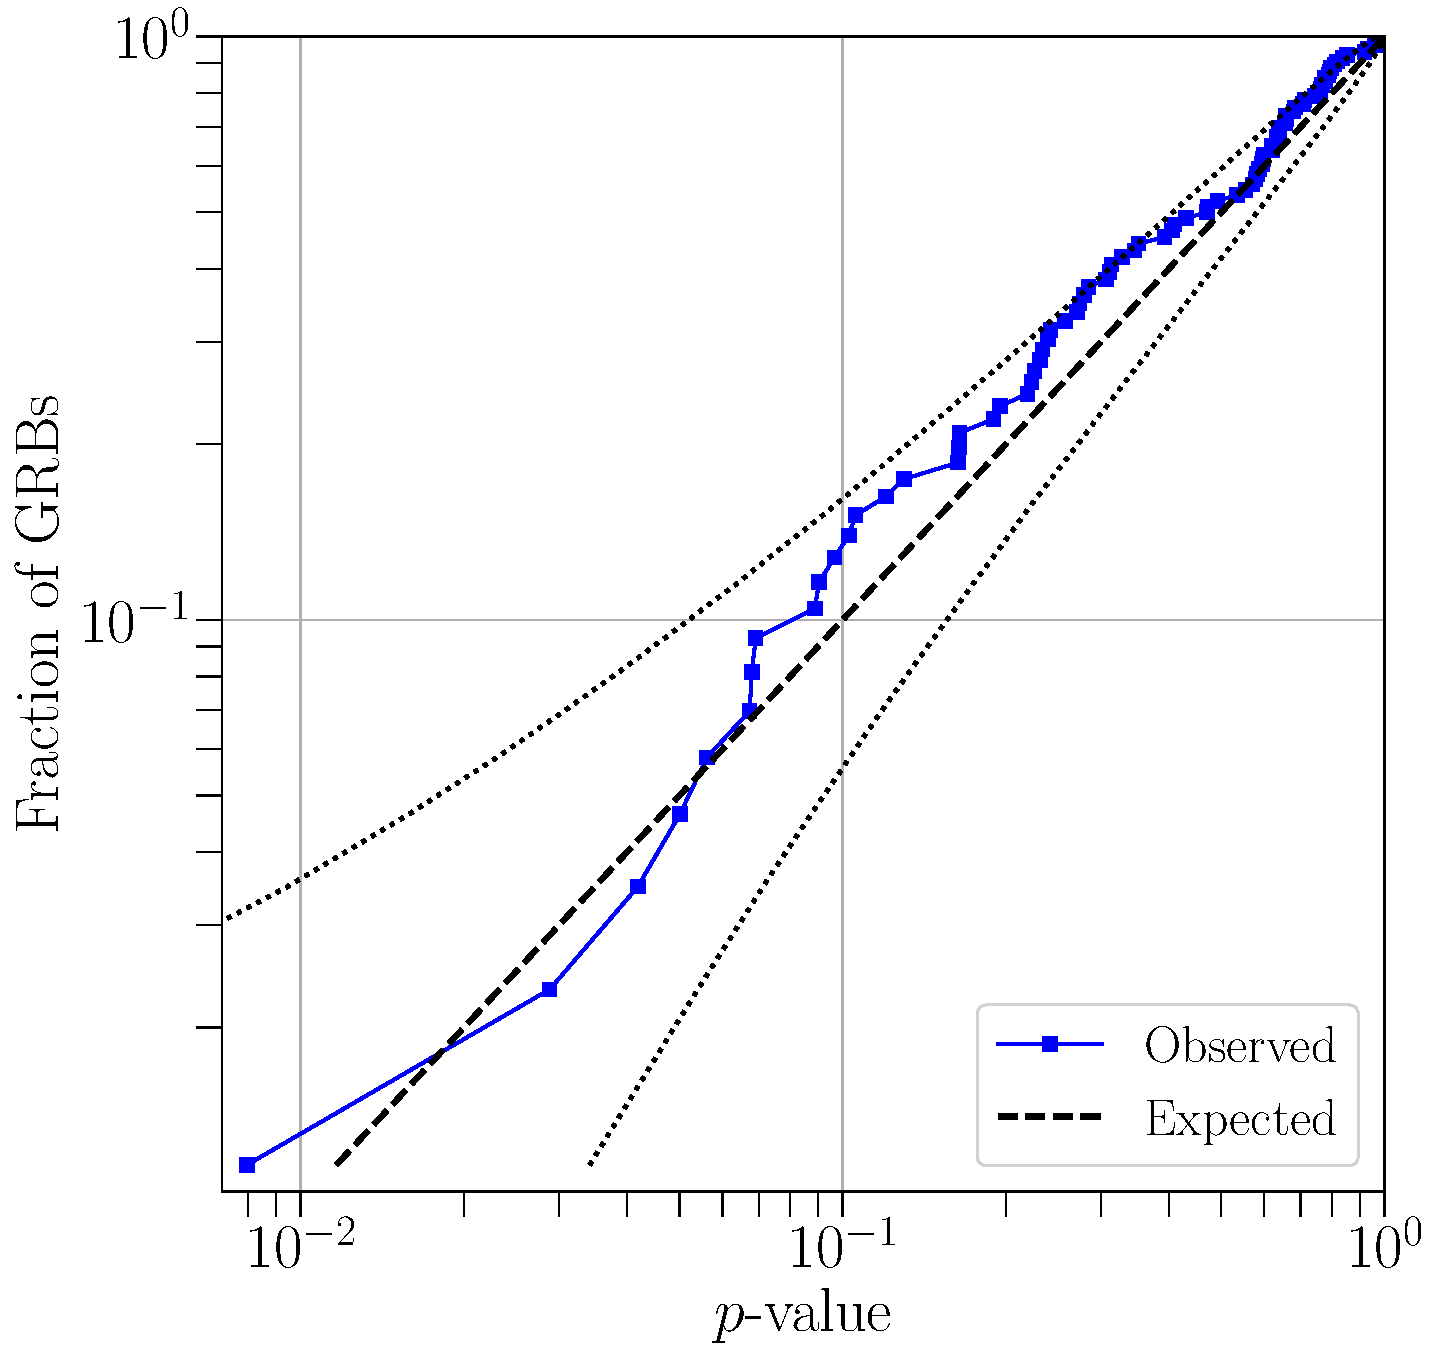
\includegraphics[width=0.7\textwidth]{figures/grb/o3b-x-pval.pdf}
  \caption
  [Cumulative distribution of p-values for the loudest on-source events of the O3b X-pipeline analyses.]
  {
    Cumulative distribution of p-values for the loudest on-source events of the O3b X-pipeline analyses.
    The dashed line indicates an expected uniform distribution of p-values under a no-signal hypothesis, with the corresponding 90\% band as the dotted lines.}
  \label{fig:grb-o3b-x-pval}
\end{figure}

Given that no loud \ac{GW} signals are observed coincident with any of the \acp{GRB} in this search, we perform a weighted binomial test to determine the probability of observing our set of p-values assuming a uniform background distribution~\citep{grb_s6}.
A small probability would suggest that there may be a population of subthreshold \ac{GW} signals that our search did not identify.
This type of weighted binomial test uses the lowest re-weighted p-values from the searches.
For the generic transient search, the test gives a probability of 0.76.
The same test carried out in O3a returned a probability of 0.30~\citep{grb_o3a}.
In \ac{O2} (removing GW170817/GRB 170817A) and the first observing run of Advanced LIGO and Advanced Virgo (O1) the probabilities were 0.75 and 0.75, respectively~\citep{grb_o2, grb_o1}.
As in these previous analyses, the probabilities obtained in O3b suggest that no weak GWs can be attributed to the population of GRBs.

\begin{figure}[h]
  \centering
  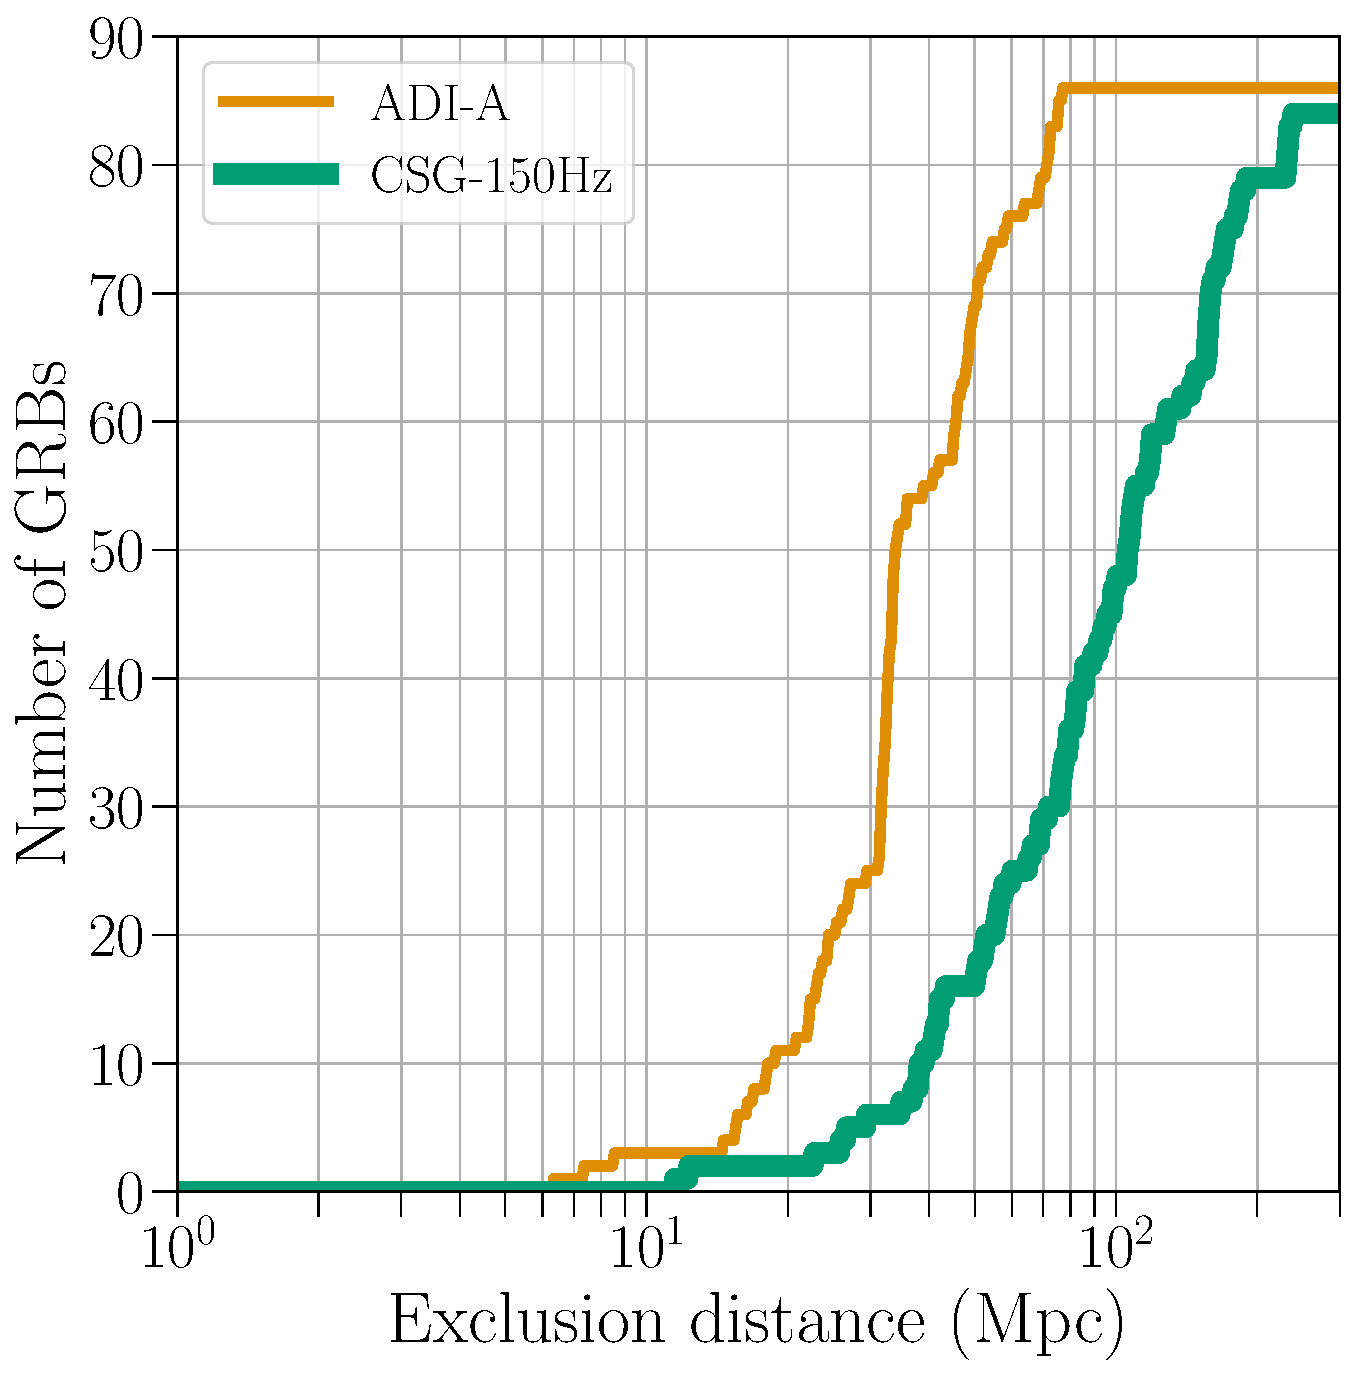
\includegraphics[width=0.7\textwidth]{figures/grb/o3b-x-exclusion.pdf}
  \caption{Cumulative distributions of O3b exclusion distances for 150-Hz sine-Gaussian and ADI-A waveforms.}
  \label{fig:grb-o3b-x-exclusion}
\end{figure}

We derive a 90\% confidence level lower limit on the distance for each of the 86 GRBs analyzed with the generic transient search, based on the different emission models.
Figure~\ref{fig:grb-o3b-x-exclusion} shows the distribution of $D_{90}$ values for the ADI-A model and for a CSG with central frequency of 150\,Hz.
The limits reported depend on the sensitivity of the instruments in the network, which change with time and sky localization of the GRB events.
We marginalize these limits over errors introduced by detector calibration.
Table~\ref{tab:grb-o3b-x-exclusion} reports the median $D_{90}$, for the set of GRBs for the different signals.
The limits vary by nearly an order of magnitude due to the variety of signals used in our analysis.
On average, the median values for the O3b generic transient search are about 50\% greater than those reported in O3a~\citep{grb_o3a}.

\begin{table}[h]
  \hspace{0.5cm}
  \caption
  {\label{tab:grb-o3b-x-exclusion} Median 90\% exclusion distances ($D_{90}$) for the generic transient search during O3b.}
  \begin{tabular}{c c c c c}
    \hline
    \hline
    \rule{0pt}{4ex}
    & CSG 70\,Hz & CSG 100\,Hz & CSG 150\,Hz & CSG 300\,Hz \\
    \hline
    \rule[-2ex]{0pt}{4ex}
    $D_{90}$ [Mpc] & 166 & 126 & 92 & 42
  \end{tabular}
  %
  \begin{tabular}{c c c c c c}
    \hline
    \hline
    \rule{0pt}{4ex}
    & ADI-A & ADI-B & ADI-C & ADI-D & ADI-E \\
    \hline
    \rule[-2ex]{0pt}{4ex}
    $D_{90}$ [Mpc] & 34 & 140 & 54 & 22 & 52 \\
    \hline
  \end{tabular}
\end{table}

We can primarily attribute this improvement to the use of autogating in O3b: the increase in exclusion distances is highest (up to a factor of 2) for the longest-duration waveforms, which are most impacted by the glitches removed by autogating.
The exclusion distances for the shorter-duration CSG waveforms, which are not expected to be affected by autogating, increased by about 30\% on average.
This is more than could be accounted for by chance differences in the LIGO–Virgo antenna factors between the two samples.
Rather, the increase is likely due to improvements in the performance of the detectors themselves, such as through the reduction of noise caused by scattered light in the LIGO detectors~\cite{Soni_2020} or the improvement in sensitivity of the Virgo detector~\cite{Davis_2021}.
% The $D_90$ values found for each GRB in the case of simulated ADI-A and 150-Hz CSG signals in Table~\ref{tab:grb-o3b-full}.


% \begin{table}
%   \caption{\label{tab:grb-o3b-full}%
%     GRB details and associated GW emission limits for
%     each of the Fermi and Swift GRBs followed up on
%     during O3b.}
%     % The GRB Name column reports each GRB's formal designation
%     % or the Fermi GBM trigger ID when a formal designation has not been assigned.
%     % The UTC times reported are rounded to the earlier integer second.
%     % The Satellite column gives the satellite that provided the
%     % GRB sky localization used in the GW analysis. The
%     % Network column lists the GW detector network used: H1 = LIGO
%     % Hanford, L1 = LIGO Livingston, V1 = Virgo.
%     % The $^\dagger$ symbol indicates that the GRB's $T_{90} > 60\,\mathrm{s}$,
%     % so the generic transient search's on-source window was extended.
%     % Where the generic transient search and the modeled search used a different
%     % IFO network, the network used by the modeled search is shown in parentheses.
%     % The last 5 columns show the 90\% confidence exclusion distances
%     % for each GRB ($D_{90}$) for the following emission scenarios:
%     % BNS, generic and aligned-spin NSBH from the modeled search,
%     % and from the generic transient search, ADI-A, and CSG
%     % GW burst at 150\,HZ with total radiated energy $E_{\text{GW}} = 10^{-2}\,\msol c^2$.}%
%   \begin{tabular}{c c c c c c c c c c c c}
%     191101A & 21:08:03 & $ 16^{\mathrm{h}} 47^{\mathrm{m}} 25^{\mathrm{s}}$ & $ 43^{\circ} 45' $ & Swift & Long & H1L1V1$^\dagger$  & 93.2 & 190.7 & 204.0 & 72.1 & 103.5 \\
191101895 & 21:28:50 & $ 10^{\mathrm{h}} 14^{\mathrm{m}} 50^{\mathrm{s}}$ & $ 18^{\circ} 58' $ & Fermi & Long & H1L1V1  & NaN & 27.0 & NaN & 25.5 & 30.0 \\
191110587 & 14:05:34 & $ 17^{\mathrm{h}} 20^{\mathrm{m}} 48^{\mathrm{s}}$ & $ 43^{\circ} 31' $ & Fermi & Long & H1L1V1  & 43.6 & 98.9 & 104.0 & 32.3 & 51.8 \\
191111347 & 08:19:09 & $  8^{\mathrm{h}} 42^{\mathrm{m}} 09^{\mathrm{s}}$ & $ -32^{\circ} 28' $ & Fermi & Long & H1L1  & 40.1 & 79.6 & 91.4 & 31.4 & 43.9 \\
191111364 & 08:44:29 & $ 12^{\mathrm{h}} 37^{\mathrm{m}} 09^{\mathrm{s}}$ & $ -32^{\circ} 07' $ & Fermi & Long & H1L1$^\dagger$  & 43.5 & 107.6 & 102.3 & 42.2 & 62.0 \\
191111547 & 13:07:10 & $ 15^{\mathrm{h}} 57^{\mathrm{m}} 38^{\mathrm{s}}$ & $ -70^{\circ} 25' $ & Fermi & Long & H1V1$^\dagger$  & 19.7 & 43.8 & 72.8 & 26.3 & 46.9 \\
191117006 & 00:08:28 & $ 19^{\mathrm{h}} 51^{\mathrm{m}} 31^{\mathrm{s}}$ & $ 76^{\circ} 23' $ & Fermi & Long & H1L1  & 78.3 & 159.8 & 144.4 & 53.7 & 82.1 \\
191117637 & 15:17:38 & $ 10^{\mathrm{h}} 29^{\mathrm{m}} 40^{\mathrm{s}}$ & $ 7^{\circ} 14' $ & Fermi & Ambiguous & H1V1  & 17.7 & 42.2 & 77.2 & 24.6 & 47.6 \\
191118925 & 22:12:01 & $ 14^{\mathrm{h}} 15^{\mathrm{m}} 57^{\mathrm{s}}$ & $ -48^{\circ} 24' $ & Fermi & Long & L1V1  & 30.1 & 69.5 & 78.3 & 22.4 & 38.8 \\
191119261 & 06:16:07 & $ 20^{\mathrm{h}} 37^{\mathrm{m}} 24^{\mathrm{s}}$ & $ -9^{\circ} 21' $ & Fermi & Long & H1L1  & 17.6 & 26.2 & 39.1 & 16.6 & 33.0 \\
191122A & 13:32:56 & $  3^{\mathrm{h}} 37^{\mathrm{m}} 09^{\mathrm{s}}$ & $ -32^{\circ} 11' $ & Swift & Long & H1L1V1$^\dagger$  & 69.8 & 146.4 & 148.3 & 49.3 & 73.3 \\
191123A & 10:38:44 & $ 14^{\mathrm{h}} 21^{\mathrm{m}} 10^{\mathrm{s}}$ & $ 22^{\circ} 50' $ & Swift & Long & L1V1$^\dagger$  & 38.4 & 92.8 & 105.1 & 32.0 & 52.4 \\
191125206 & 04:56:43 & $ 16^{\mathrm{h}} 12^{\mathrm{m}} 21^{\mathrm{s}}$ & $ -13^{\circ} 07' $ & Fermi & Long & H1L1V1$^\dagger$  & 86.4 & 180.3 & 176.9 & 59.1 & 94.1 \\
191125634 & 15:12:45 & $ 23^{\mathrm{h}} 34^{\mathrm{m}} 09^{\mathrm{s}}$ & $ 18^{\circ} 12' $ & Fermi & Long & H1L1V1  & 53.6 & 110.1 & 104.3 & 34.7 & 65.2 \\
191129141 & 03:22:27 & $  0^{\mathrm{h}} 35^{\mathrm{m}} 43^{\mathrm{s}}$ & $ 5^{\circ} 26' $ & Fermi & Long & L1V1  & 22.2 & 52.6 & 68.6 & 34.2 & 68.8 \\
191130253 & 06:04:41 & $ 23^{\mathrm{h}} 17^{\mathrm{m}} 36^{\mathrm{s}}$ & $ 63^{\circ} 05' $ & Fermi & Long & H1V1$^\dagger$  & 15.8 & 39.7 & 60.2 & 23.7 & 49.7 \\
191130507 & 12:09:34 & $ 23^{\mathrm{h}} 14^{\mathrm{m}} 24^{\mathrm{s}}$ & $ -7^{\circ} 44' $ & Fermi & Long & L1V1$^\dagger$  & 21.7 & 56.5 & 74.0 & 36.3 & 70.3 \\
191130A & 13:05:02 & $  8^{\mathrm{h}} 52^{\mathrm{m}} 19^{\mathrm{s}}$ & $ 4^{\circ} 60' $ & Swift & Long & L1V1  & 25.9 & 57.9 & 94.6 & 32.6 & 53.5 \\
191202867 & 20:48:51 & $ 16^{\mathrm{h}} 38^{\mathrm{m}} 08^{\mathrm{s}}$ & $ 17^{\circ} 33' $ & Fermi & Long & H1L1V1  & 86.8 & 173.6 & 182.9 & 69.7 & 95.0 \\
191203290 & 06:57:19 & $ 22^{\mathrm{h}} 09^{\mathrm{m}} 33^{\mathrm{s}}$ & $ 51^{\circ} 49' $ & Fermi & Short & H1L1  & 19.1 & 51.0 & 72.7 & 32.0 & 42.9 \\
191205741 & 17:46:20 & $  0^{\mathrm{h}} 56^{\mathrm{m}} 09^{\mathrm{s}}$ & $ -34^{\circ} 09' $ & Fermi & Ambiguous & H1L1  & 74.9 & 158.7 & 146.2 & 58.0 & 77.0 \\
191213A & 04:06:23 & $ 14^{\mathrm{h}} 58^{\mathrm{m}} 07^{\mathrm{s}}$ & $ -9^{\circ} 45' $ & Swift & Long & H1L1V1$^\dagger$  & 79.7 & 161.7 & 39.1 & 51.1 & 54.9 \\
191213254 & 06:05:33 & $ 13^{\mathrm{h}} 04^{\mathrm{m}} 14^{\mathrm{s}}$ & $ -30^{\circ} 27' $ & Fermi & Long & H1L1V1  & 64.0 & 120.3 & 83.6 & 49.7 & 72.1 \\
191213784 & 18:49:07 & $ 22^{\mathrm{h}} 04^{\mathrm{m}} 14^{\mathrm{s}}$ & $ -13^{\circ} 56' $ & Fermi & Long & H1L1V1  & 6.7 & 22.9 & 20.4 & 8.6 & 1.0 \\
191220A & 13:29:37 & $ 18^{\mathrm{h}} 45^{\mathrm{m}} 20^{\mathrm{s}}$ & $ 26^{\circ} 40' $ & Swift & Long & L1V1$^\dagger$  & 37.8 & 79.6 & 94.5 & 32.7 & 52.7 \\
191220589 & 14:08:29 & $ 14^{\mathrm{h}} 07^{\mathrm{m}} 04^{\mathrm{s}}$ & $ -67^{\circ} 31' $ & Fermi & Long & L1V1  & 21.8 & 57.0 & 74.4 & 22.5 & 46.7 \\
191221B & 20:39:13 & $ 10^{\mathrm{h}} 19^{\mathrm{m}} 19^{\mathrm{s}}$ & $ -38^{\circ} 09' $ & Swift & Long & H1V1$^\dagger$  & 29.4 & 69.7 & 105.0 & 33.8 & 68.4 \\
191225309 & 07:25:16 & $  6^{\mathrm{h}} 21^{\mathrm{m}} 57^{\mathrm{s}}$ & $ -17^{\circ} 21' $ & Fermi & Long & L1V1$^\dagger$  & 17.4 & 41.0 & 92.1 & 31.8 & 52.2 \\
191225735 & 17:37:51 & $  9^{\mathrm{h}} 43^{\mathrm{m}} 12^{\mathrm{s}}$ & $ -7^{\circ} 11' $ & Fermi & Long & H1L1$^\dagger$  & 16.2 & 34.9 & 44.1 & 32.0 & 48.0 \\
191227A & 01:39:37 & $ 21^{\mathrm{h}} 16^{\mathrm{m}} 40^{\mathrm{s}}$ & $ -16^{\circ} 43' $ & Swift & Long & H1V1$^\dagger$  & 39.8 & 83.4 & 98.3 & 31.6 & 46.9 \\
191227723 & 17:21:44 & $ 17^{\mathrm{h}} 12^{\mathrm{m}} 40^{\mathrm{s}}$ & $ -26^{\circ} 01' $ & Fermi & Short & H1L1V1  & 56.8 & 119.6 & 128.8 & 45.7 & 68.1 \\
191228A & 00:01:19 & $  0^{\mathrm{h}} 21^{\mathrm{m}} 27^{\mathrm{s}}$ & $ -8^{\circ} 41' $ & Swift & Long & H1L1V1$^\dagger$  & 79.1 & 164.1 & 148.2 & 52.1 & 76.5 \\
200101861 & 20:39:26 & $ 17^{\mathrm{h}} 09^{\mathrm{m}} 43^{\mathrm{s}}$ & $ -35^{\circ} 04' $ & Fermi & Long & L1V1  & 27.4 & 65.6 & 70.2 & 18.3 & 37.6 \\
200103678 & 16:16:50 & $ 23^{\mathrm{h}} 41^{\mathrm{m}} 31^{\mathrm{s}}$ & $ -38^{\circ} 22' $ & Fermi & Long & H1V1  & NaN & NaN & 35.6 & 15.7 & 30.2 \\
200103689 & 16:32:23 & $  7^{\mathrm{h}} 53^{\mathrm{m}} 55^{\mathrm{s}}$ & $ -0^{\circ} 54' $ & Fermi & Long & H1L1V1$^\dagger$  & 9.0 & NaN & 27.2 & 18.0 & 31.6 \\
200105914 & 21:55:28 & $ 21^{\mathrm{h}} 32^{\mathrm{m}} 07^{\mathrm{s}}$ & $ -41^{\circ} 11' $ & Fermi & Long & H1L1V1  & 37.5 & 78.3 & 73.6 & 23.1 & 43.5 \\
200109A & 01:46:16 & $ 20^{\mathrm{h}} 28^{\mathrm{m}} 27^{\mathrm{s}}$ & $ 52^{\circ} 59' $ & Swift & Long & L1V1$^\dagger$  & 18.9 & 56.0 & 79.7 & 24.7 & 40.3 \\
200110518 & 12:26:08 & $  6^{\mathrm{h}} 24^{\mathrm{m}} 36^{\mathrm{s}}$ & $ 28^{\circ} 53' $ & Fermi & Long & H1V1$^\dagger$  & 18.3 & 41.7 & 60.5 & 22.2 & 38.4 \\
200112395 & 09:28:27 & $ 12^{\mathrm{h}} 27^{\mathrm{m}} 52^{\mathrm{s}}$ & $ -34^{\circ} 19' $ & Fermi & Long & H1L1V1  & 54.0 & 106.2 & 95.5 & 36.1 & 56.6 \\
200112525 & 12:36:31 & $ 10^{\mathrm{h}} 00^{\mathrm{m}} 31^{\mathrm{s}}$ & $ 64^{\circ} 25' $ & Fermi & Long & H1L1V1  & 69.5 & 139.2 & 141.3 & 45.4 & 78.2 \\
200114153 & 03:40:43 & $ 13^{\mathrm{h}} 17^{\mathrm{m}} 31^{\mathrm{s}}$ & $ -0^{\circ} 19' $ & Fermi & Long & H1L1V1  & 64.3 & 156.5 & 141.1 & 48.1 & 72.8 \\
200115A & 11:50:23 & $  3^{\mathrm{h}} 45^{\mathrm{m}} 48^{\mathrm{s}}$ & $ 5^{\circ} 36' $ & Swift & Long & H1L1$^\dagger$  & 53.8 & 108.1 & 102.1 & 33.6 & 52.1 \\
200117517 & 12:24:06 & $  8^{\mathrm{h}} 38^{\mathrm{m}} 40^{\mathrm{s}}$ & $ -62^{\circ} 31' $ & Fermi & Long & H1L1V1  & 47.9 & 108.3 & 98.6 & 27.1 & 40.1 \\
200120962 & 23:04:55 & $  9^{\mathrm{h}} 08^{\mathrm{m}} 32^{\mathrm{s}}$ & $ -70^{\circ} 26' $ & Fermi & Long & H1V1  & 34.9 & 77.1 & 105.1 & 46.5 & 71.5 \\
200122A & 01:41:00 & $ 14^{\mathrm{h}} 00^{\mathrm{m}} 02^{\mathrm{s}}$ & $ 27^{\circ} 33' $ & Swift & Long & H1L1V1$^\dagger$  & 43.6 & 106.5 & 101.2 & 32.4 & 48.7 \\
200122221 & 05:18:20 & $  8^{\mathrm{h}} 18^{\mathrm{m}} 38^{\mathrm{s}}$ & $ 67^{\circ} 05' $ & Fermi & Ambiguous & H1L1V1  & 79.3 & 170.3 & 162.1 & 41.3 & 58.1 \\
200125864 & 20:43:31 & $  0^{\mathrm{h}} 29^{\mathrm{m}} 47^{\mathrm{s}}$ & $ 64^{\circ} 41' $ & Fermi & Long & H1L1  & 80.7 & 172.1 & 175.7 & 68.9 & 87.1 \\
200126466 & 11:10:51 & $  3^{\mathrm{h}} 57^{\mathrm{m}} 52^{\mathrm{s}}$ & $ -59^{\circ} 37' $ & Fermi & Short & L1V1  & 13.5 & 38.3 & 102.1 & 23.3 & 65.6 \\
200127758 & 18:11:18 & $  5^{\mathrm{h}} 03^{\mathrm{m}} 33^{\mathrm{s}}$ & $ 20^{\circ} 04' $ & Fermi & Long & H1L1  & 43.6 & 99.8 & 95.1 & 33.1 & 49.2 \\
200128153 & 03:40:05 & $ 10^{\mathrm{h}} 34^{\mathrm{m}} 36^{\mathrm{s}}$ & $ 41^{\circ} 34' $ & Fermi & Short & L1V1  & 24.9 & 60.6 & 93.6 & 27.4 & 50.5 \\
200129409 & 09:48:44 & $ 23^{\mathrm{h}} 05^{\mathrm{m}} 07^{\mathrm{s}}$ & $ -44^{\circ} 58' $ & Fermi & Short & H1L1V1  & 116.1 & 236.0 & 202.7 & 64.5 & 90.3 \\
200130248 & 05:57:16 & $ 21^{\mathrm{h}} 57^{\mathrm{m}} 09^{\mathrm{s}}$ & $ -65^{\circ} 56' $ & Fermi & Long & H1V1  & 18.5 & 42.4 & 110.4 & 33.9 & 71.0 \\
200130417 & 09:59:56 & $  9^{\mathrm{h}} 10^{\mathrm{m}} 07^{\mathrm{s}}$ & $ -51^{\circ} 20' $ & Fermi & Long & H1L1  & NaN & 11.5 & 14.1 & 6.4 & 9.8 \\
200131A & 22:41:15 & $  0^{\mathrm{h}} 12^{\mathrm{m}} 21^{\mathrm{s}}$ & $ 51^{\circ} 07' $ & Swift & Long & H1L1V1  & 115.0 & 235.4 & 212.8 & 77.8 & 109.3 \\
200201040 & 00:57:20 & $ 19^{\mathrm{h}} 10^{\mathrm{m}} 50^{\mathrm{s}}$ & $ -11^{\circ} 02' $ & Fermi & Long & H1L1V1  & 37.4 & 86.2 & 101.7 & 33.7 & 54.5 \\
200205845 & 20:17:23 & $ 14^{\mathrm{h}} 52^{\mathrm{m}} 50^{\mathrm{s}}$ & $ -42^{\circ} 47' $ & Fermi & Long & H1L1  & 68.6 & 157.6 & 142.0 & 50.3 & 73.9 \\
200207058 & 01:22:55 & $ 16^{\mathrm{h}} 16^{\mathrm{m}} 21^{\mathrm{s}}$ & $ -48^{\circ} 18' $ & Fermi & Long & L1V1  & 20.9 & 50.4 & 71.0 & 31.9 & 58.5 \\
200208052 & 01:14:17 & $  1^{\mathrm{h}} 46^{\mathrm{m}} 55^{\mathrm{s}}$ & $ 25^{\circ} 19' $ & Fermi & Long & L1V1  & 37.0 & 76.6 & 95.1 & 45.5 & 68.3 \\
200211310 & 07:26:28 & $ 23^{\mathrm{h}} 00^{\mathrm{m}} 48^{\mathrm{s}}$ & $ -7^{\circ} 09' $ & Fermi & Long & H1L1$^\dagger$  & 86.0 & 182.9 & 188.4 & 71.8 & 100.8 \\
200212451 & 10:49:49 & $  8^{\mathrm{h}} 19^{\mathrm{m}} 11^{\mathrm{s}}$ & $ 22^{\circ} 57' $ & Fermi & Long & H1L1  & 40.8 & 86.4 & 94.0 & 33.9 & 49.6 \\
200215A & 14:39:31 & $  2^{\mathrm{h}} 16^{\mathrm{m}} 24^{\mathrm{s}}$ & $ 12^{\circ} 47' $ & Swift & Long & H1V1  & 41.6 & 90.1 & 101.1 & 33.3 & 54.1 \\
200216380 & 09:07:25 & $ 20^{\mathrm{h}} 45^{\mathrm{m}} 45^{\mathrm{s}}$ & $ -11^{\circ} 39' $ & Swift & Long & H1L1V1  & 80.2 & 159.4 & 155.0 & 51.3 & 75.0 \\
200216B & 13:32:33 & $ 10^{\mathrm{h}} 41^{\mathrm{m}} 49^{\mathrm{s}}$ & $ 19^{\circ} 28' $ & Swift & Long & H1L1V1$^\dagger$  & 37.6 & 77.2 & 93.3 & 32.7 & 48.5 \\
200219A & 07:36:49 & $ 22^{\mathrm{h}} 50^{\mathrm{m}} 22^{\mathrm{s}}$ & $ -59^{\circ} 06' $ & Swift & Long & H1L1V1$^\dagger$  & 112.7 & 232.1 & 215.4 & 75.8 & 108.3 \\
200219413 & 09:54:14 & $ 19^{\mathrm{h}} 56^{\mathrm{m}} 31^{\mathrm{s}}$ & $ 6^{\circ} 39' $ & Fermi & Long & H1L1V1  & 57.2 & 119.0 & 121.7 & 46.4 & 69.1 \\
200221162 & 03:52:58 & $ 10^{\mathrm{h}} 28^{\mathrm{m}} 24^{\mathrm{s}}$ & $ 33^{\circ} 08' $ & Fermi & Ambiguous & H1L1V1  & 68.7 & 157.7 & 152.5 & 54.9 & 84.7 \\
200223814 & 19:32:03 & $ 16^{\mathrm{h}} 33^{\mathrm{m}} 33^{\mathrm{s}}$ & $ -55^{\circ} 47' $ & Fermi & Long & L1V1$^\dagger$  & 37.6 & 81.9 & 102.5 & 33.0 & 53.2 \\
200224A & 03:24:49 & $ 16^{\mathrm{h}} 34^{\mathrm{m}} 58^{\mathrm{s}}$ & $ 41^{\circ} 40' $ & Swift & Long & H1L1  & 5.7 & 12.3 & 10.0 & 7.4 & 10.7 \\
200224212 & 05:05:49 & $ 11^{\mathrm{h}} 51^{\mathrm{m}} 36^{\mathrm{s}}$ & $ -28^{\circ} 52' $ & Fermi & Long & H1L1V1$^\dagger$  & 45.5 & 94.2 & 94.4 & 34.3 & 50.3 \\
200224416 & 09:58:44 & $ 12^{\mathrm{h}} 28^{\mathrm{m}} 04^{\mathrm{s}}$ & $ -19^{\circ} 33' $ & Fermi & Short & H1L1V1  & 50.1 & 110.6 & 111.9 & 32.6 & 53.9 \\
200227A & 07:20:08 & $  3^{\mathrm{h}} 45^{\mathrm{m}} 43^{\mathrm{s}}$ & $ 9^{\circ} 29' $ & Swift & Long & H1L1V1  & 26.8 & 67.0 & 69.2 & 21.0 & 33.4 \\
200228291 & 06:58:33 & $ 21^{\mathrm{h}} 52^{\mathrm{m}} 02^{\mathrm{s}}$ & $ -46^{\circ} 27' $ & Fermi & Ambiguous & H1L1V1  & 118.3 & 241.2 & 231.4 & 76.3 & 107.9 \\
200228B & 11:14:41 & $ 16^{\mathrm{h}} 48^{\mathrm{m}} 01^{\mathrm{s}}$ & $ 16^{\circ} 58' $ & Swift & Long & H1L1  & 84.9 & 185.1 & 203.2 & 72.8 & 104.3 \\
200301320 & 07:40:46 & $ 21^{\mathrm{h}} 20^{\mathrm{m}} 33^{\mathrm{s}}$ & $ 7^{\circ} 30' $ & Fermi & Long & H1L1V1  & 63.8 & 149.6 & 154.7 & 48.5 & 73.5 \\
200303A & 02:34:57 & $ 14^{\mathrm{h}} 10^{\mathrm{m}} 47^{\mathrm{s}}$ & $ 51^{\circ} 22' $ & Swift & Long & H1L1V1$^\dagger$  & 45.2 & 96.2 & 100.5 & 29.6 & 49.2 \\
200306934 & 22:25:25 & $ 23^{\mathrm{h}} 18^{\mathrm{m}} 07^{\mathrm{s}}$ & $ 5^{\circ} 06' $ & Fermi & Ambiguous & L1V1  & 3.6 & 29.8 & 27.9 & 19.0 & 33.8 \\
200306C & 22:50:39 & $ 13^{\mathrm{h}} 14^{\mathrm{m}} 18^{\mathrm{s}}$ & $ 11^{\circ} 16' $ & Swift & Long & L1V1$^\dagger$  & 29.9 & 72.4 & 100.7 & 31.8 & 44.1 \\
200307894 & 21:26:59 & $  5^{\mathrm{h}} 36^{\mathrm{m}} 43^{\mathrm{s}}$ & $ -46^{\circ} 13' $ & Fermi & Ambiguous & H1L1  & 41.0 & 83.3 & 96.2 & 33.9 & 49.0 \\
200308941 & 22:35:15 & $ 21^{\mathrm{h}} 49^{\mathrm{m}} 45^{\mathrm{s}}$ & $ -27^{\circ} 45' $ & Fermi & Long & H1L1V1  & 57.1 & 115.9 & 124.4 & 39.3 & 68.8 \\
200311636 & 15:16:12 & $ 13^{\mathrm{h}} 35^{\mathrm{m}} 57^{\mathrm{s}}$ & $ -49^{\circ} 41' $ & Fermi & Long & H1L1  & 61.2 & 129.4 & 132.7 & 49.1 & 70.5 \\
200313071 & 01:41:36 & $  5^{\mathrm{h}} 03^{\mathrm{m}} 09^{\mathrm{s}}$ & $ 20^{\circ} 53' $ & Fermi & Long & H1L1V1  & 115.0 & 232.3 & 210.0 & 72.8 & 100.9 \\
200317028 & 00:40:30 & $  4^{\mathrm{h}} 22^{\mathrm{m}} 09^{\mathrm{s}}$ & $ -46^{\circ} 19' $ & Fermi & Long & H1L1V1  & 25.4 & 53.0 & 54.1 & 15.6 & 34.1 \\
200319323 & 07:44:40 & $  4^{\mathrm{h}} 21^{\mathrm{m}} 09^{\mathrm{s}}$ & $ -21^{\circ} 15' $ & Fermi & Long & H1L1  & 57.5 & 128.2 & 136.6 & 47.1 & 71.9 \\
200320414 & 09:56:46 & $ 12^{\mathrm{h}} 17^{\mathrm{m}} 21^{\mathrm{s}}$ & $ -38^{\circ} 44' $ & Fermi & Long & H1L1V1  & 23.1 & 37.1 & 43.8 & 14.7 & 34.2 \\
200323006 & 00:08:42 & $ 22^{\mathrm{h}} 56^{\mathrm{m}} 50^{\mathrm{s}}$ & $ 53^{\circ} 02' $ & Fermi & Long & L1V1  & 14.4 & 38.3 & 61.8 & 17.1 & 32.8 \\
200326517 & 12:24:47 & $ 16^{\mathrm{h}} 21^{\mathrm{m}} 19^{\mathrm{s}}$ & $ -21^{\circ} 05' $ & Fermi & Long & H1L1V1$^\dagger$  & 46.0 & 101.0 & 104.1 & 33.2 & 52.3 \\

%   \end{tabular}
% \end{table}


\subsection{Model exclusion}\label{sec:grb-o3b-models}

Although \xpip is an entirely unmodeled \ac{GW} search pipeline, given the substantial improvement in the exclusion distances in O3b, we may be approaching the point at which extreme GW emission models can be excluded using out null results and the sensitivity estimates for injected waveforms.
Using detection efficiency curves of both the O3a and O3b searches, we can compute for each model an exclusion confidence using the method described in~\citet{Kalmus_2013} for supernova searches~\citep{burst_o2}.
The model exclusion probability given $N$ targeted GRBs is

\begin{equation}
	P_{\text{excl}} = 1 - \prod_{i=1}^N \left[ 1 - \varepsilon_i(d_i) \right]
\end{equation}
where $\varepsilon_i(d_i)$ is the detection efficiency at the source distance of $d_i$.
Of the 86 GRBs analyzed in the O3b search by \xpip, only one, GRB 191221B has a redshift measurement (GRB 200205B did not occur at a time when at least two detectors were active and was therefore not included).
For the remaining GRBs, we have no distance measurement, but instead we can sample $d_i$ from the distribution of redshifts measured by Swift \ac{BAT}.

\begin{figure}[h]
  \centering
  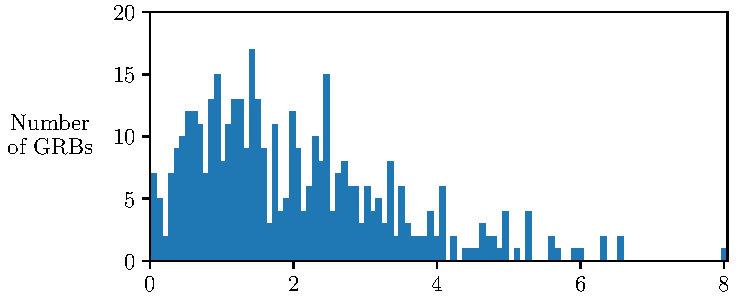
\includegraphics{figures/grb/redshifts.pdf}
  \caption{Histogram of redshift measurements for GRBs detected by Swift BAT.}
  \label{fig:grb-o3b-redshifts}
\end{figure}

The Swift GRB archive has redshift measurements for 411 triggers~\cite{swift_archive}.
Figure~\ref{fig:grb-o3b-redshifts} shows the distribution of those measurements, from which we sample distances for the 86 GRBs analyzed, using inverse transform sampling, and compute exclusion probability for each model.
This is repeated 1,000 times and $P_{\text{excl}}$ is averaged for each model across all trials.

\begin{table}[h]
  \hspace{0.5cm}
  \caption
  {\label{tab:grb-o3b-model-exclusion} Exclusion confidence for each injected waveform model.}
  \begin{tabular}{c c c c c}
    \hline
    \hline
    \rule{0pt}{4ex}
    & CSG 70\,Hz & CSG 100\,Hz & CSG 150\,Hz & CSG 300\,Hz \\
    \hline
    \rule[-2ex]{0pt}{4ex}
		$P_{\text{excl}}$ & \textbf{0.74} & \textbf{0.63} & 0.44 & 0.12
  \end{tabular}
  %
  \begin{tabular}{c c c c c c}
    \hline
    \hline
    \rule{0pt}{4ex}
    & ADI-A & ADI-B & ADI-C & ADI-D & ADI-E \\
    \hline
    \rule[-2ex]{0pt}{4ex}
    $P_{\text{excl}}$ & 0.04 & \textbf{0.61} & 0.15 & 0.00 & 0.18 \\
    \hline
  \end{tabular}
\end{table}

The averages are presented in Table~\ref{tab:grb-o3b-model-exclusion}.
The model with the highest exclusion probability is the 70-Hz sine-Gaussian model.
Assuming that the Swift redshift distribution is representative of the GRBs analyzed by \xpip, it is more likely than not that we can rule out the very optimistic energies simulated by the low-frequency 70-Hz and 100-Hz sine-Gaussian injections ($E_{\text{GW}} = 10^{-2}\,\msol c^2$) based on the lack of GW-GRB joint detections at O3 sensitivity.

If search sensitivity continues to improve in \ac{O4}, we may well be able to begin ruling out the most extreme emission models.
The exclusion probability for the ADI-B model is 0.61, making it the only unfavorable ADI model so far.
This accretion disk instability model is simulated for a central \ac{BH} mass of $M=10\,\msol$, a dimensionless spin parameter of $\chi=0.95$, and a very large clump mass of $\epsilon=0.2$ times that the central \ac{BH}.
It is the most extreme of the ADI models, and it would not be surprising to see it being ruled out in future searches.


\subsection{Noise effects in the generic transient search}\label{sec:grb-o3b-noise}

Comparing the exclusion distances of the O3a and O3b search sheds some light on the impact of detector and search pipeline improvements on the sensitivity of the \xpip analysis.
Table~\ref{tab:grb-o3b-compare-o3a} presents the improvement in the median $D_{90}$ for each waveform model as a fraction of the O3a value.
% Two-sample Kolmogorov-Smirnov tests conducted between the O3a and O3b $D_{90}$ distributions for each model show very low p-values for all of them, clearnly rejecting the null hypothesis that the data are drawn from the same distribution.
Given the large number of GRBs analyzed, it would be unlikely for the difference to be explained by chance improvement in antenna response (i.e. due to more GRBs lining up with the sky region where the GW detector network is most sensitive).
\xpip reports the antenna response of the GW detectors for each GRB analyzed.
These can be summed up over the active detectors for each GRB and averaged over the full GRB sample.
The result is a 9.2\% improvement in antenna response, which is not negligible but can only account for a small portion of the differences in exclusion distances.

\begin{table}[h]
  \hspace{0.5cm}
  \caption
  {\label{tab:grb-o3b-compare-o3a} Relative increase in median $D_{90}$ for each \xpip simulated waveform.}
  \begin{tabular}{c c c c c}
    \hline
    \hline
    \rule{0pt}{4ex}
    & CSG 70\,Hz & CSG 100\,Hz & CSG 150\,Hz & CSG 300\,Hz \\
    \hline
    \rule[-2ex]{0pt}{4ex}
		$\Delta D_{90} / D_{90, \text{O3a}}$ & 0.12 & 0.19 & 0.25 & 0.49
  \end{tabular}
  %
  \begin{tabular}{c c c c c c}
    \hline
    \hline
    \rule{0pt}{4ex}
    & ADI-A & ADI-B & ADI-C & ADI-D & ADI-E \\
    \hline
    \rule[-2ex]{0pt}{4ex}
    $\Delta D_{90} / D_{90, \text{O3a}}$ & 0.43 & 0.14 & 0.85 & 0.92 & 0.55 \\
    \hline
  \end{tabular}
\end{table}

For the longest duration ADI-C, ADI-D, and ADI-E waveforms, we see the greatest improvements, over 50\% higher than in O3a (Figure~\ref{fig:grb-o3b-compare-o3a}, top).
For short-duration waveforms, the highest-frequency 300-Hz sine-Gaussian injections show the greatest change (Figure~\ref{fig:grb-o3b-compare-o3a}, bottom).
These are all well above the change expected from a chance difference in antenna response.

\begin{figure}[h]
  \centering
  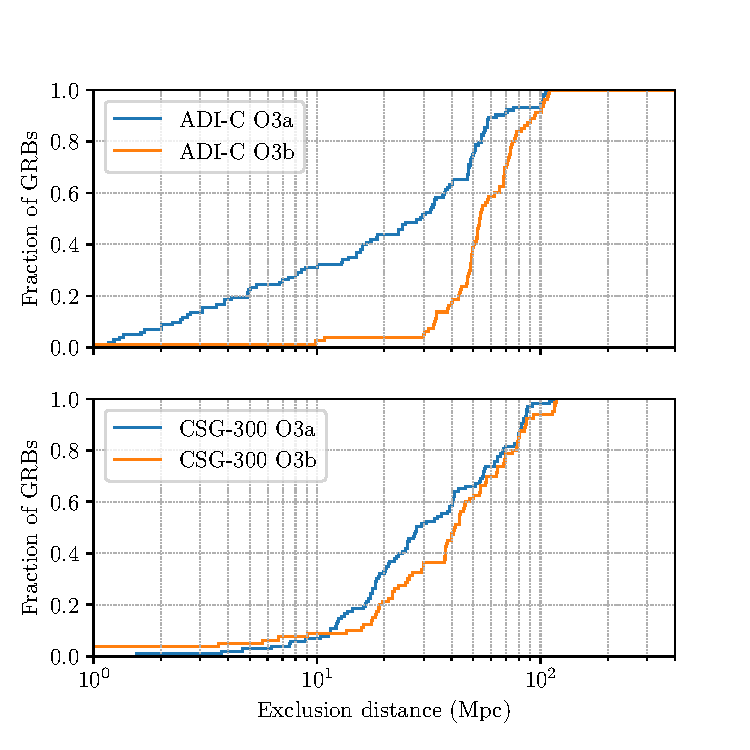
\includegraphics{figures/grb/compare-o3a.pdf}
  \caption
	[Cumulative distributions of O3a and O3b exclusion distances for the ADI-C (top) and 300-Hz sine-Gaussian (bottom) waveforms.]
	{Cumulative distributions of O3a and O3b exclusion distances for the ADI-C (top) and 300-Hz sine-Gaussian (bottom) waveforms.
	These show the greatest improvement between O3a and O3b among their respective waveform sets.}
  \label{fig:grb-o3b-compare-o3a}
\end{figure}

Considering that longer-duration waveforms see greater improvement, the most obvious likely contributor is the implementation of autogating.
However, autogating cannot account for the changes in the $D_{90}$ of short-duration models.
These can only be explained by better GW detector sensitivity and/or reduced rates of short-duration glitches that overlap the injected signal.
Such glitches cause the entire injection to be vetoed, so it is not recovered by the search pipeline.
In particular, glitches caused by low-frequency scattering noise (such as those discussed in Section~\ref{sec:vib}) can pepper a stretch of time with short-duration glitches, overlapping injections made at multiple points.
A method for reducing the occurrence of these glitches, \ac{RC} tracking, was implemented at for O3b, on Jan 7, 2020 at \ac{LLO} and Jan 15, 2020~\citep{Soni_2020}.

\begin{figure}[h]
  \centering
  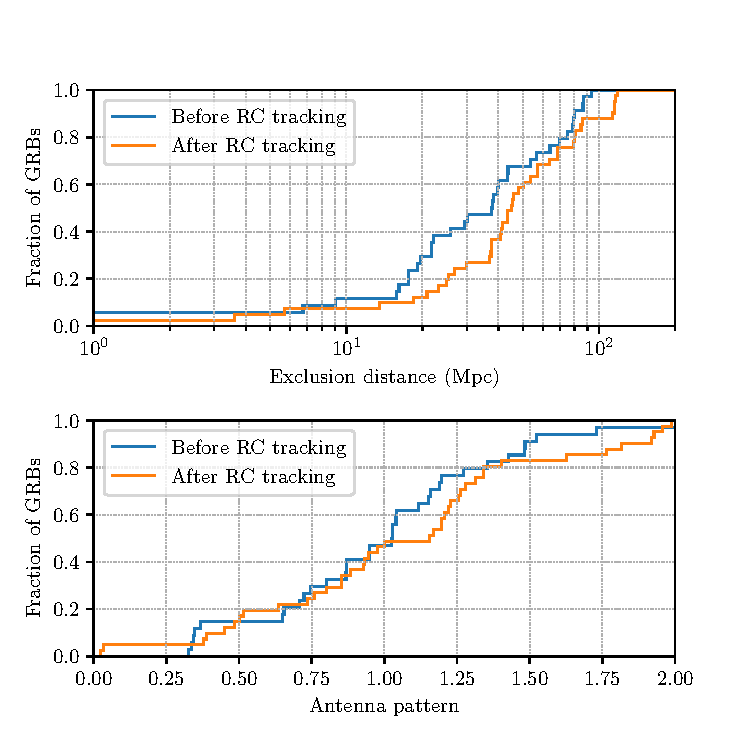
\includegraphics{figures/grb/compare-rc.pdf}
  \caption
	{Cumulative distributions of CSG-300 Hz exclusion distances (top) and the detector network antenna factors (bottom) for GRBs before and after the implementation of RC tracking.}
  \label{fig:grb-o3b-compare-rc}
\end{figure}

Figure~\ref{fig:grb-o3b-compare-rc} gives evidence for the effect of glitch mitigation on \xpip sensitivity.
Although there is clearly a bias towards higher antenna responses after RC tracking, they do not entirely account for the huge substantial increase in exclusion distances.
In summary, noise mitigation is a crucial part of improving the sensitivity of the generic transient search.
As discussed above, there may plenty that can be inferred even in the absence of detections.
Better detector sensitivities in \ac{O4}, along with the development of new glitch subtraction methods, could allow more confident exclusion of GW emission models associated with GRBs.
